
The architecture of our system, called Text2KB, is presented on Figure \ref{fig:model}. 
The left part of the picture roughly corresponds to the architecture of existing information extraction approaches to knowledge base question answering.
The right part introduces additional different external text data sources, which are integrated into the question answering pipeline on multiple stages.
In this work we use web search results, community question answering (CQA) data and we use a large collection of documents with detected KB entity mentions.
But besides external text data, many knowledge bases including Freebase contain some text data as well.
In Freebase most of the entities contain a description paragraph, which often comes from the entity Wikipedia profile.
These descriptions of entities in the KB were found useful for text-based question answering \cite{Sun:2015:ODQ:2736277.2741651}.
For completeness, we decided to include them in our system as well.
Each description is represented as a vector of tokens and as a vector of mentioned entities and we compute a cosine similarity between the question tokens and entity vectors and use these scores as features for candidate ranking.
In a similar we can incorporate any other entity profile text, such as full Wikipedia article.

\subsection{Web search results}
\label{section:method:web}

We start by issuing a question as a query to a commercial web search engine\footnote{https://datamarket.azure.com/dataset/bing/search} and extract top 10 search result snippets and get the corresponding documents.
Document snippets are usually built to present the information most relevant to the query and often contain answers to a question.
Unfortunately, for longer queries the snippets often represent and combination of small phrases, that contain mostly question terms and very few additional information.
Nevertheless, we keep both snippets and documents text, and using system's linker detect KB entity mentions.
This data turns out to be useful for multiple purposes, \ie question entity identification and answer candidate ranking.

\textbf{Question entity identification}.
Question text provides a very limited context for entity disambiguation and in addition the entity name can be misspelled or an uncommon variation can be used.
This complicates question topical entity identification, which is the foundation of whole question answering process.
Luckily, web search results help with these problems as they usually contain multiple various mentions of the same entities and provide more context for disambiguation.

To extend the set of detected question entities Text2KB uses search results snippets.
There are multiple mentions of different entities, to filter out only entities, that are also mentioned in the question we use string distance.
More specifically, we take names of all entities detected in the question and compute their term by term similarity with non-stopwords from the question.
In this work we used Jaro-Winkler string distance and and entity was added to the list of question entities if at least one of its tokens $e_t$ have high similarity with one of the question tokens $q_t$ excluding stopwords ($Stop$), \ie:
$$\max_{\begin{split}e_t \in M\backslash Stop\\ q_t \in Q\backslash Stop\end{split}} distance_{Jaro-Winkler}(e_t, q_t) \geq 0.8$$

\textbf{Answer candidate features}.
Most of the information stored in knowledge bases is also present in other formats, including natural language statements, tables, \etc
For example, on Figure \ref{fig:web_search_entitylink} multiple snippets mention the date when Tutankhamun became the king.
Text-based question answering system usually generate answer candidates from passages extracted from retrieved documents.
In our case candidates are already generated in a form of KB queries, that return certain subsets of entities.
Text2KB uses snippets and documents to compute a set of features, which are used for answer candidate ranking.
More specifically we do this following:
\begin{enumerate}
\setlength\itemsep{-0.5em}
\item Precompute term and entity IDFs\footnote{https://en.wikipedia.org/wiki/Tf-idf}. We used Google n-grams corpus to approximate terms IDF by collection frequency and available ClueWeb Freebase entity annotations\footnote{http://lemurproject.org/clueweb09/FACC1/} to compute entity IDFs
\item Each snippet and document is represented by two TF-IDF vectors of lowercased tokens and mentioned entities
\item In addition, vectors of all snippets and all documents are merged together to form combined token and entity vectors
\item Each answer candidate is also represented as TF-IDF vectors of terms (from entity names) and entities
\item We compute cosine similarities between answer and each snippet and document token and entity vectors. This gives us 10 similarity scores for every document for token vectors and 10 similarities for entity vectors, we take average and maximum scores as features.
\item We do the same for the combined document and use cosine similarities as features
\end{enumerate}

\subsection{Community Question Answering data}
\label{section:method:cqa}

Manual labeling of questions with answers is expensive and therefore largest KBQA datasets still contain just several thousands of examples, which is too small for data intensive approaches to learn good strategies for mapping questions into millions of KB entities and predicates.
Researchers have proposed to use weakly supervised methods to extend the lexicon with mappings learned from statements mentioning entity pairs from a large corpus \cite{yao2014information}.
However, often there exist a lexical gap between how information is asked about in a question and how it is expressed in a statement.
On the other hand there are huge archives of questions and answers posted by real users on various community question answering websites, \eg Figure \ref{fig:cqa_example}.

\begin{figure}
\centering
\fbox{
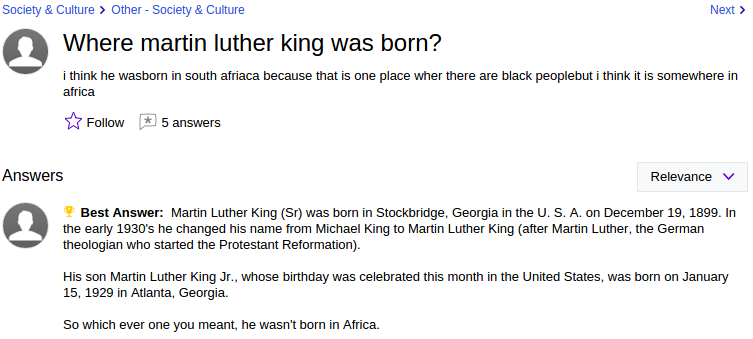
\includegraphics[width=0.45\textwidth]{img/cqa_example}
}
\caption{Example of a question and answer pair from Yahoo! Answers}
\label{fig:cqa_example}
\end{figure}

For our experiments we took 4,483,032 questions from Yahoo! Comprehensive Questions and Answers WebScope dataset\footnote{https://webscope.sandbox.yahoo.com/catalog.php?datatype=l}.
Texts of each question and answer pair were run through an entity linker, that detected mentions of Freebase entities.
Next, similar to an idea of relation extraction from CQA data \cite{savenkov-EtAl:2015:SRW}, we use distant supervision to label each question-answer pair with relations between entities mentioned in the question and in the answer.
As a result we have a set of questions, annotated with KB predicates connecting some question and answer entities, which are, often incorrectly, assumed to answer the question.
We learn associations between question terms and predicates by computing pointwise mutual information scores\footnote{https://en.wikipedia.org/wiki/Pointwise\_mutual\_information} (PMI) for each term-predicate pair.
Examples of scores for some terms from WebQuestions dataset questions are given in Table \ref{table:cqa_npmi}.

\begin{table}
\caption{Examples of term-predicate pairs with high PMI scores}
\label{table:cqa_npmi}
\begin{tabular}{| p{1cm} | p{5.5cm} | p{0.75cm} |}
\hline
Term & Predicate & PMI score\\
\hline
born & people.person.date\_of\_birth & 3.67\\
 & people.person.date\_of\_death & 2.73\\
 & location.location.people\_born\_here & 1.60\\
\hline
kill & people.deceased\_person.cause\_of\_death & 1.70\\
& book.book.characters & 1.55\\
\hline
currency & location.country.currency\_formerly\_used & 5.55 \\
& location.country.currency\_used & 3.54 \\
\hline
school & education.school.school\_district & 4.14 \\
& people.education.institution & 1.70\\
& sports.school\_sports\_team.school & 1.69 \\
\hline
illness & medicine.symptom.symptom\_of & 2.11\\
& medicine.decease.causes & 1.68\\
& medicine.disease.treatments & 1.59\\
\hline
win & sports.sports\_team.championships & 4.11\\
& sports.sports\_league.championship & 3.79\\
\hline
\end{tabular}
\end{table}

Although noisy, the statistics look reasonable to be used for candidate ranking.
In Text2KB we take candidate answer predicates and lookup PMI scores between these predicates and terms in the question.
Missing pairs are given a score of 0, and minimum, average and maximum of these scores are used as features.
Since this kind of data is usually sparse, we decided to consider vector space embeddings of terms to solve a problem of synonym terms with missing score.
We use pretrained word2vec word embeddings\footnote{https://code.google.com/p/word2vec/} to generate predicate embeddings by taking weighted average of term vectors from predicate's PMI table.
Each term's embedding vector is weighted by its PMI value (terms with negative score are skipped).
Then, we compute cosine similarities between predicate vector and question term vectors and take their minimum, average, maximum as features.
Similarity between the predicate vector and average question term vector is also computed.


\subsection{Entity pair language model}
\label{section:method:clueweb}

When ranking candidate answer, we are interested in estimating if topic and answer entities are related in a way asked in the question.
Existing systems usually look on how candidate predicates are expressed in questions and statements.
But predicate isn't the only way we can look at this, another alternative is to consider text pieces, \eg sentences, that mention topical and answer entities together.
For example, in the bottom right corner of Figure \ref{fig:model} we can see some passages that mentioned a pair of people, and the context of these mentions often expresses the nature of the relationships between the entities.
This resembles OpenQA approach of \cite{Fader:2014:OQA:2623330.2623677} with a difference, that information isn't filtered out by keeping only some sentences and converting them to a triple format.
Moreover, since these relationships are now expressed in a natural language, we can consider various measures of text similarity between them and the question.

We take ClueWeb12 corpus with existing Freebase entity annotations\footnote{http://lemurproject.org/clueweb12/FACC1/} and compute counts of different terms that occur in the context to an entity pair mention.
By an entity pair mention we mean a pair of mentions of different entities within 200 characters of each other.
We take terms in between mentions and 100 character before and after mentions as the context.
A small sample of this data is presented in Table \ref{table:clueweb_entitypairs_langmodel}.

\begin{table}
\caption{Examples of entity pairs language model data}
\label{table:clueweb_entitypairs_langmodel}
\begin{tabular}{| p{1.25cm} | p{1.23cm} | p{4.5cm} |}
\hline
Entity 1 & Entity 2 & Term counts\\
\hline
John Edwards & Rielle Hunter & campaign, affair, mistress, child, former ...\\
\hline
John Edwards & Cate Edwards & daughter, former, senator, courthouse, left, greensboro, eldest ...\\
\hline
John Edwards & Elizabeth Edwards & wife, hunter, campaign, affair, cancer, rielle, husband ...\\
\hline
John Edwards & Frances Quinn Hunter & daughter, john, rielle, father, child, former, paternity...\\
\hline
\end{tabular}
\end{table}

First, given a set of question terms $Q$, an answer candidate, that includes question entity $e_1$, we compute a language model score for every answer entity $e_2$:
$$p(Q|e_1, e_2) = \prod_{t\in Q} p(t | e_1, e_2)$$
and use minimum, average and maximum as features.
Similar to the way we handled CQA-based data, we use embeddings to handle the sparsity problem.
For each entity pair a weighted (by counts) average embedding vector of terms is computed and again minimum, average and maximum cosine similarities between this vectors and question tokens vector is used as features.

%\subsubsection{Wikipedia profile}
%It would be nice to have Wikipedia pages for entities and use something like SDM score or something else as feature.